\section{Computing framework}
\label{sec:Framework}

A computing framework that automates the \rich mirror software alignment
procedure was developed. It is based on \ganga~\cite{Mościcki20092303}, a tool
for computational-task management and easy access to Grid resources. A schematic
workflow diagram is shown in \fig{fig:workflow}.

\begin{figure}
  \vspace{-0.5\baselineskip}
  \centering
  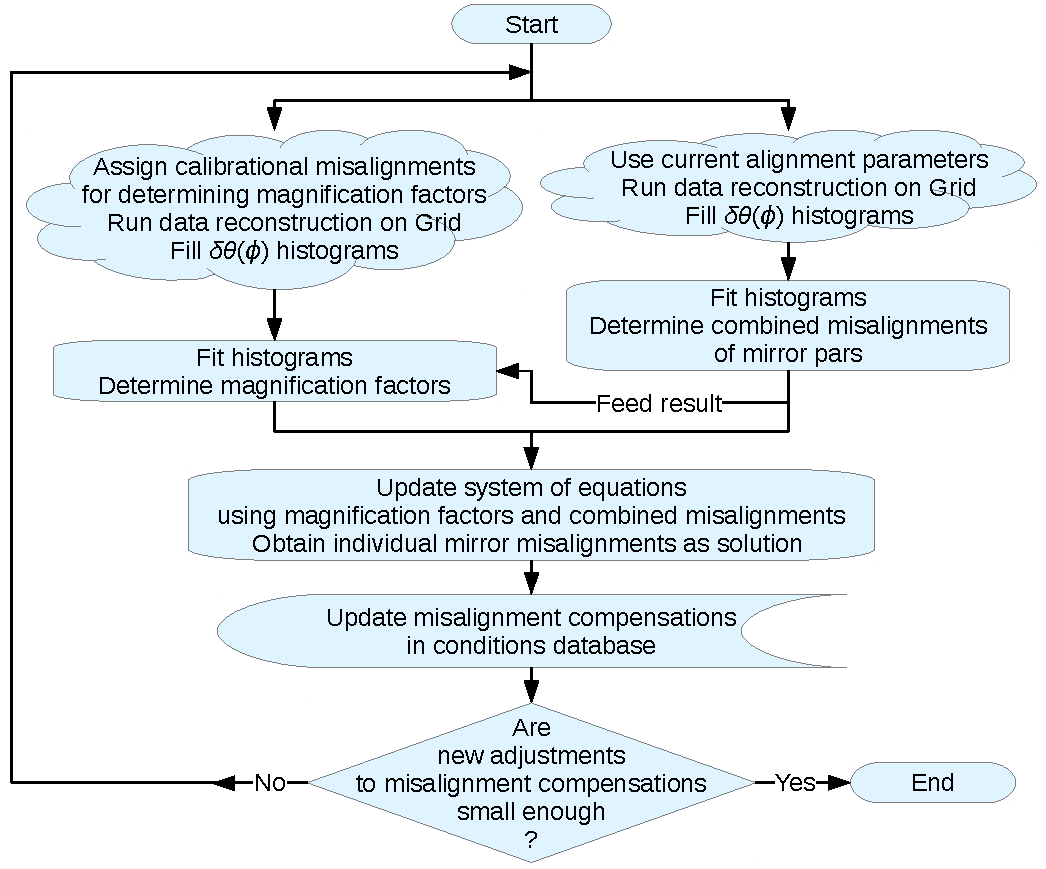
\includegraphics[width=1.0\textwidth]{figs/Framework/Workflow.pdf}
  \vspace{-1.0\baselineskip}
  \caption{
    Schematic diagram of the computing framework workflow steered by the \ganga
    script.}
  \label{fig:workflow}
  \vspace{-0.5\baselineskip}
\end{figure}

Currently, this software facility consists of a steering \ganga script, written
in Python, and three programs written in C++: a module that fills the
$\deltatheta(\phi)$ histograms necessary for determining possible mirror
misalignments while running the reconstruction over the preselected events
(see~\sect{sec:SelectionMethod}); a program that for every mirror combination
from the chosen subset finds combined tilts resulting from misalignments of both
primary and secondary mirror segments and a program that determines individual
misalignment compensating corrections for every mirror segment of both mirror
kinds.

This script runs a loop of iterations, each consisting of the following actions:
\begin{enumerate}
  \item
  run multiple data reconstruction jobs parallelized by \ganga across the Grid
  and produce $\delta\theta(\phi)$ histograms for every combination of one
  spherical and one flat mirror according to the optimized list of combinations
  determined in advance; this bunch of jobs forks into two groups, each running
  over the same set of DSTs but using different misalignment compensation
  values:
  \begin{enumerate}
    \item
    just up-to-date values
    \item
    additional calibrational tilts (e.g. $\pm 0.3\mrad$) are added to the
    up-to-date values of only one member of a combination at a time, for all
    combinations, in order to determine the magnification factors
    (see~\sect{subsec:Magnification})
  \end{enumerate}
  \item
  fit these histograms and determine for each combination its combined tilts
  around $y$- as well as $z$-axis in two case:
  \begin{enumerate}
    \item
    just as they are
    \item
    resulting from additional calibrational tilts
  \end{enumerate}
  \item
  magnification factors are calculated by dividing difference between biased
  combined tilts and the unbiased ones by the corresponding calibrational tilts
  \item
  update the system of linear equations using obtained magnification factors and
  total tilts; its solution is a set of individual tilts (around $y$ and $z$) of
  every segment
  \item
  update the existing misalignment compensations in CONDDB that were used during
  the current iteration
  \item
  if all the obtained adjustments to the previous misalignment corrections are
  (by absolute value) less than 0.1\unit{\mrad}, exit; otherwise continue.
\end{enumerate}
Because contents of CONDDB is stored in XML, we used Xerces-C++~\cite{Xerces311}
XML parser and XQilla~\cite{XQilla230} as an XQuery and XPath implementation to
alter the RICH mirror alignment adjustments in CONDDB.
